In the previous parts we presented mathematical tools for the theoretical interpretation of amplitudes in field theory and string theory.
The ultimate goal of the analysis is to provide some insights on the predictive capabilities of the string theory framework applied to phenomenological data.
As already argued in~\Cref{sec:CYmanifolds} the procedure is however quite challenging as there are different ways to match string theory with the experimental reality, that is there are several different vacuum configurations arising from the compactification of the extra-dimensions.
The investigation of feasible phenomenological models in a string framework has therefore to deal also with computational aspects related to the exploration of the \emph{landscape}~\cite{Douglas:2003:StatisticsStringTheory} of possible vacua.
Unfortunately the number of possibilities is huge (numbers as high as $\num{e272000}$ have been suggested for some models)~\cite{Lerche:1987:ChiralFourdimensionalHeterotic, Douglas:2003:StatisticsStringTheory, Ashok:2004:CountingFluxVacua, Douglas:2004:BasicResultsVacuum, Douglas:2007:FluxCompactification, Taylor:2015:FtheoryGeometryMost, Schellekens:2017:BigNumbersString, Halverson:2017:AlgorithmicUniversalityFtheory, Taylor:2018:ScanningSkeleton4D, Constantin:2019:CountingStringTheory}, the mathematical objects entering the compactifications are complex and typical problems are often NP-complete, NP-hard, or even undecidable~\cite{Denef:2007:ComputationalComplexityLandscape, Halverson:2019:ComputationalComplexityVacua, Ruehle:2020:DataScienceApplications}, making an exhaustive classification impossible.
Additionally, there is no single framework to describe all the possible (flux) compactifications.
As a consequence, each class of models must be studied with different methods.
This has prevented any precise connection to the existing and tested theories (in particular, the \sm of particle physics).

Until recently the string landscape has been studied using different methods such as analytic computations for simple examples, general statistics, random scans or algorithmic enumerations of possibilities.
This has been a large endeavor of the string community~\cite{Grana:2006:FluxCompactificationsString, Lust:2009:SeeingStringLandscape, Ibanez:2012:StringTheoryParticle, Brennan:2018:StringLandscapeSwampland, Halverson:2018:TASILecturesRemnants, Ruehle:2020:DataScienceApplications}.
The main objective of such studies is to understand what are the generic predictions of string theory.
The first conclusion of these studies is that compactifications giving an effective theory close to the Standard Model are scarce~\cite{Dijkstra:2005:ChiralSupersymmetricStandard, Dijkstra:2005:SupersymmetricStandardModel, Blumenhagen:2005:StatisticsSupersymmetricDbrane, Gmeiner:2006:OneBillionMSSMlike, Douglas:2007:LandscapeIntersectingBrane, Anderson:2014:ComprehensiveScanHeterotic}.
The approach however has limitations mainly given by lack of a general understanding or high computational power required to run the algorithms.

In reaction to these difficulties and starting with the seminal paper~\cite{Abel:2014:GeneticAlgorithmsSearch} new investigations based on Machine Learning (\ml) appeared in the recent years, focusing on different aspects of the string landscape and of the geometries used in compactifications~\cite{Krefl:2017:MachineLearningCalabiYau, Ruehle:2017:EvolvingNeuralNetworks, He:2017:MachinelearningStringLandscape, Carifio:2017:MachineLearningString, Altman:2019:EstimatingCalabiYauHypersurface, Bull:2018:MachineLearningCICY, Cole:2019:TopologicalDataAnalysis, Klaewer:2019:MachineLearningLine, Mutter:2019:DeepLearningHeterotic, Wang:2018:LearningNonHiggsableGauge, Ashmore:2019:MachineLearningCalabiYau, Brodie:2020:MachineLearningLine, Bull:2019:GettingCICYHigh, Cole:2019:SearchingLandscapeFlux, Faraggi:2020:MachineLearningClassification, Halverson:2019:BranesBrainsExploring, He:2019:DistinguishingEllipticFibrations, Bies:2020:MachineLearningAlgebraic, Bizet:2020:TestingSwamplandConjectures, Halverson:2020:StatisticalPredictionsString, Krippendorf:2020:DetectingSymmetriesNeural, Otsuka:2020:DeepLearningKmeans, Parr:2020:ContrastDataMining, Parr:2020:PredictingOrbifoldOrigin} (see also~\cite{Erbin:2018:GANsGeneratingEFT, Betzler:2020:ConnectingDualitiesMachine, Chen:2020:MachineLearningEtudes, Gan:2017:HolographyDeepLearning, Hashimoto:2018:DeepLearningAdS, Hashimoto:2018:DeepLearningHolographic, Hashimoto:2019:AdSCFTCorrespondence, Tan:2019:DeepLearningHolographic, Akutagawa:2020:DeepLearningAdS, Yan:2020:DeepLearningBlack, Comsa:2019:SupergravityMagicMachine, Krishnan:2020:MachineLearningGauged} for related works and~\cite{Ruehle:2020:DataScienceApplications} for a comprehensive summary of the state of the art).
In fact \ml is definitely adequate when it comes to pattern search or statistical inference starting from large amount of data.
This motivates two main applications to string theory: the systematic exploration of the space of possibilities (if they are not random then \ml should be able to find a pattern) and the deduction of mathematical formulas from the \ml approximation.
The last few years have seen a major uprising of \ml, and more particularly of neural networks (\nn)~\cite{Bengio:2017:DeepLearning, Chollet:2018:DeepLearningPython, Geron:2019:HandsOnMachineLearning}.
This technology is efficient at discovering and predicting patterns and now pervades most fields of applied sciences and of the industry.
One of the most critical places where progress can be expected is in understanding the geometries used to describe string compactifications and this will be the object of study in the following analysis.

We address the question of computing the Hodge numbers $\hodge{1}{1} \in \N$ and $\hodge{2}{1} \in \N$ for \emph{complete intersection Calabi--Yau} (\cicy) $3$-folds~\cite{Green:1987:CalabiYauManifoldsComplete} using different \ml algorithms.
A \cicy is completely specified by its \emph{configuration matrix} (whose entries are positive integers) which is the basic input of the algorithms.
The \cicy $3$-folds are the simplest manifolds of their kind and they have been well studied.
In particular they have been completely classified and their topological properties computed~\cite{Candelas:1988:CompleteIntersectionCalabiYau, Green:1989:AllHodgeNumbers, Anderson:2017:FibrationsCICYThreefolds}.
For these reasons, they provide an excellent sandbox to test \ml algorithms in a controlled environment.

The goal is therefore to predict two positive integers from a matrix of positive integers.
This task is complicated by various redundancies in the description (such as an independence in the permutations of lines and columns).
While usual physics application of \ml reduces to feeding a (big) sequential neural network with raw data, real-world applications are built following a more general pipeline~\cite{Geron:2019:HandsOnMachineLearning, Skiena:2017:DataScienceDesign}.
In fact the first task after understanding of the problem would be to perform and exploratory data analysis (\eda) to highlight possible data which may help in getting a result.
After the definition of a validation strategy, feature engineering can be used to improve the baseline computations and improve the design of \ml models.
While the first step is straightforward it is still interesting to notice that computations involved in string geometries (using algebraic topology) are far from standard applications of \ml algorithms, which makes the problem even more interesting.
\eda aims at better understanding the dataset showing how the variables are distributed, correlated, determining if outliers are present, etc.
This analysis naturally leads to designing new variables during \emph{feature engineering} which can be used in addition (or even substitution) of the original data.
Adding derived features by hand may make the data more easily understandable by the \ml algorithms for instance by emphasizing important properties.\footnotemark{}
\footnotetext{%
  While one could expect \ml algorithms to generate these features by themselves, this may complicate the learning process.
  So in cases where it is straightforward to compute meaningful derived features it is often worth considering them.
}
This phase is followed by \emph{feature selection}, where different set of features are chosen according to the need of each algorithm.
A good validation strategy is also needed to ensure that the predictions appropriately reflect the real values, together with a baseline model, which gives a lower bound on the accuracy together with a working pipeline.\footnotemark{}
\footnotetext{%
  For example the original work on this topic~\cite{He:2017:MachinelearningStringLandscape} did not set up a validation strategy and reported the accuracy over both the training and test data.
  Correcting this problem leads to an accuracy of $37\%$~\cite{Bull:2018:MachineLearningCICY}.
}
For instance, we find that a simple linear regression using the configuration matrix as input gives \SIrange{43.6}{48.8}{\percent} for \hodge{1}{1} and \SIrange{9.6}{10.4}{\percent} for \hodge{2}{1} using from $20\%$ to $80\%$ of data for training.
Hence any algorithm \emph{must} do better than this to be worth considering.

In the dataset we use for accomplishing the task there is a finite number of $7890$ \cicy $3$-folds.
Due to the freedom in representing the configuration matrix, two datasets have been constructed: the \emph{original dataset}~\cite{Candelas:1988:CompleteIntersectionCalabiYau, Green:1989:AllHodgeNumbers} and the \emph{favourable dataset}~\cite{Anderson:2017:FibrationsCICYThreefolds}.
Our analysis continues and generalises~\cite{He:2017:MachinelearningStringLandscape, Bull:2018:MachineLearningCICY} at different levels.
For example we compute \hodge{2}{1} which has been ignored in~\cite{He:2017:MachinelearningStringLandscape, Bull:2018:MachineLearningCICY}, where the authors argue that it can be computed from \hodge{1}{1} and from the Euler characteristics (a simple formula exists for the latter).
In our case, we want to push the idea of using \ml to learn about the physics (or the mathematics) of \cy to its very end: we assume that we do not know anything about the mathematics of the \cicy, except that the configuration matrix is sufficient to derive all quantities.
Moreover we have already mentioned that \ml algorithms have rarely been used to derive data in algebraic topology, which can be a difficult task.
Thus getting also \hodge{2}{1} from \ml techniques is an important first step towards using ML for more general problems in string geometries.
Finally regression is also more useful for extrapolating results: a classification approach assumes that we already know all the possible values of the Hodge numbers and has difficulties to predict labels which do not appear in the training set.
This is necessary when we move to a dataset for which not all topological quantities have been computed, for instance CY constructed from the Kreuzer--Skarke list of polytopes~\cite{Kreuzer:2000:CompleteClassificationReflexive}.

The data analysis and \ml are programmed in Python using standard open-source packages: \texttt{pandas}~\cite{WesMcKinney:2010:DataStructuresStatistical}, \texttt{matplotlib}~\cite{Hunter:2007:Matplotlib2DGraphics}, \texttt{seaborn}~\cite{Waskom:2020:MwaskomSeabornV0}, \texttt{scikit-learn}~\cite{Pedregosa:2011:ScikitlearnMachineLearning}, \texttt{scikit-optimize}~\cite{Head:2020:ScikitoptimizeScikitoptimize}, \texttt{tensorflow}~\cite{Abadi:2015:TensorFlowLargescaleMachine} (and its high level API \emph{Keras}).
The code and its description are available on \href{https://thesfinox.github.io/ml-cicy/}{Github}.


\subsection{Complete Intersection Calabi--Yau Manifolds}
\label{sec:data:cy}

As presented in~\Cref{sec:CYmanifolds}, a \cy $n$-fold is a $n$-dimensional complex manifold $X$ with \SU{n} holonomy (dimension in \R is $2n$).
An equivalent definition is the vanishing of its first Chern class.
A standard reference for the physicist is~\cite{Hubsch:1992:CalabiyauManifoldsBestiary} (see also~\cite{Anderson:2018:TASILecturesGeometric, He:2020:CalabiYauSpacesString} for useful references).
The compactification on a \cy leads to the breaking of large part of the supersymmetry which is phenomenologically more realistic than the very high energy description with intact supersymmetry.

Calabi--Yau manifolds are characterised by a certain number of topological properties (see~\Cref{sec:cohomology_hodge}), the most salient being the Hodge numbers \hodge{1}{1} and \hodge{2}{1}, counting respectively the Kähler and complex structure deformations, and the Euler characteristics:\footnotemark{}
\footnotetext{%
  In full generality, the Hodge numbers \hodge{p}{q} count the numbers of harmonic $\qty(p,\, q)$-forms.
}%
\begin{equation}
  \chi = 2 \qty(\hodge{1}{1} - \hodge{2}{1}).
  \label{eq:cy:euler}
\end{equation}
Interestingly, topological properties of the manifold directly translates into features of the $4$-dimensional effective action (in particular, the number of fields, the representations and the gauge symmetry)~\cite{Hubsch:1992:CalabiyauManifoldsBestiary, Becker:2006:StringTheoryMTheory}.\footnotemark{}
\footnotetext{%
	Another reason for sticking to topological properties is that there is no CY for which the metric is known.
	Hence, it is not possible to perform explicitly the Kaluza--Klein reduction in order to derive the $4$-dimensional theory.
}%
In particular, the Hodge numbers count the number of chiral multiplets (in heterotic compactifications) and the number of hyper- and vector multiplets (in type II compactifications): these are related to the number of fermion generations ($3$ in the Standard Model) and is thus an important measure of the distance to the Standard Model.

The simplest CYs are constructed by considering the complete intersection of hypersurfaces in a product $\cA$ of projective spaces $\mathds{P}^{n_i}$ (called the ambient space)~\cite{Green:1987:CalabiYauManifoldsComplete, Green:1987:PolynomialDeformationsCohomology, Candelas:1988:CompleteIntersectionCalabiYau, Green:1989:AllHodgeNumbers, Anderson:2017:FibrationsCICYThreefolds, Anderson:2018:TASILecturesGeometric}:
\begin{equation}
  \cA = \mathds{P}^{n_1} \times \cdots \times \mathds{P}^{n_m}.
\end{equation}
Such hypersurfaces are defined by homogeneous polynomial equations: a Calabi--Yau $X$ is described by the solution to the system of equations, i.e.\ by the intersection of all these surfaces.
The intersection is ``complete'' in the sense that the hypersurface is non-degenerate.

To gain some intuition, consider the case of a single projective space $\mathds{P}^n$ with (homogeneous) coordinates $Z^I$, $I = 0, \ldots, n$.
A codimension $1$ subspace is obtained by imposing a single homogeneous polynomial equation of degree $a$ on the coordinates:
\begin{equation}
  \begin{split}
    p_a\qty(Z^0,\, \dots,\, Z^n)
    & =
    P_{I_1 \dots I_a}\, Z^{I_1} \dots Z^{I_a}
    = 0,
    \\
    p_a\qty(\lambda Z^0,\, \dots,\, \lambda Z^n)
    & =
    \lambda^a \, p_a\qty(Z^0,\, \dots,\, Z^n).
  \end{split}
\end{equation}
Each choice of the polynomial coefficients $P_{I_1 \dots I_a}$ leads to a different manifold.
However it can be shown that the manifolds are in general topologically equivalent.
Since we are interested only in classifying the \cy as topological manifolds and not as complex manifolds, the information on $P_{I_1 \dots I_a}$ can be discarded and it is sufficient to keep track only of the dimension $n$ of the projective space and of the degree $a$ of the equation.
The resulting hypersurface is denoted equivalently as $\qty[\mathds{P}^n \mid a] = \qty[n \mid a]$.
Notice that $\qty[\mathds{P}^n \mid a]$ is $3$-dimensional if $n = 4$ (the equation reduces the dimension by one), and it is a \cy (the ``quintic'') if $a = n + 1 = 5$ (this is required for the vanishing of its first Chern class).
The simplest representative of this class if Fermat's quintic defined by the equation:
\begin{equation}
  \finitesum{I}{0}{4} \qty( Z^I )^5 = 0.
\end{equation}

This construction can be generalized to include $m$ projective spaces and $k$ equations which can mix the coordinates of the different spaces.
A \cicy $3$-fold $X$ as a topological manifold is completely specified by a \emph{configuration matrix} denoted by the same symbol as the manifold:
\begin{equation}
  X =
  \left[
    \begin{array}{c|ccc}
      \mathds{P}^{n_1} & a_1^1 & \cdots & a_k^1
      \\
      \vdots & \vdots & \ddots & \vdots
      \\
      \mathds{P}^{n_m} & a_1^m & \cdots & a_k^m
    \end{array}
  \right]
\end{equation}
where the coefficients $a^r_{\alpha}$ are positive integers and satisfy the following constraints
\begin{equation}
  \dim_{\C} X = \finitesum{r}{1}{m} n_r - k = 3,
  \qquad
  n_r + 1 = \sum_{\alpha=1}^k a_\alpha^r,
  \quad
  \forall r \in \qty{1,\, 2,\, \dots,\, m}.
  \label{eq:cicy-constraints}
\end{equation}
The first relation states that the difference between the dimension of the ambient space and the number of equations is the dimension of the \cy $3$-fold.
The second set of constraints arises from the vanishing of its first Chern class.
It implies that the $n_i$ can be recovered from the matrix elements.
Two manifolds described by the same configuration matrix but different polynomials are diffeomorphic as real manifold, and thus as topological manifolds, but they are different as complex manifolds.
Hence it makes sense to write only the configuration matrix.

A given topological manifold is not described by a unique configuration matrix.
First, any permutation of the lines and columns leave the intersection unchanged as it amounts to relabelling the projective spaces and equations.
Secondly, two intersections can define the same manifold.
The ambiguity in the line and column permutations is often fixed by imposing some ordering of the coefficients.
Moreover there is an optimal representation of the manifold $X$, called \emph{favourable}~\cite{Anderson:2017:FibrationsCICYThreefolds}: in such form topological properties of $X$ can be more conveniently derived from the ambient space $\cA$.
Finally, simple arguments~\cite{Green:1987:CalabiYauManifoldsComplete, Candelas:1988:CompleteIntersectionCalabiYau, Lutken:1988:RecentProgressCalabiYauology} show that the number of \cicy is necessarily finite due to the constraints~\eqref{eq:cicy-constraints} together with identities between complete intersection manifolds.


\subsection{Datasets}
\label{sec:data:datasets}

The classification of the \cicy $3$-folds has been tackled in~\cite{Candelas:1988:CompleteIntersectionCalabiYau}.
The analysis established a dataset of $7890$ \cicy.
The topological properties of each of these manifolds have been computed in~\cite{Green:1989:AllHodgeNumbers}.
More recently a new classification has been performed~\cite{Anderson:2017:FibrationsCICYThreefolds} in order to find the favourable representation of each manifold whenever it is possible.

Below we show a list of the \cicy properties and of their configuration matrices:
\begin{itemize}
  \item general properties:
  \begin{itemize}
    \item number of configurations: $7890$
    \item number of product spaces (block diagonal matrix): $22$
    \item $h^{11} \in [0, 19]$ with $18$ distinct values (\Cref{fig:data:hist-h11})
    \item $h^{21} \in [0, 101]$ with $65$ distinct values (\Cref{fig:data:hist-h21})
    \item unique Hodge number combinations: $266$
  \end{itemize}

  \item ``original dataset''~\cite{Candelas:1988:CompleteIntersectionCalabiYau, Green:1989:AllHodgeNumbers}
  \begin{itemize}
    \item maximal size of the configuration matrices: $12 \times 15$
    \item number of favourable matrices (excluding product spaces): $4874$ ($\num{61.8}\%$)
    \item number of non-favourable matrices (excluding product spaces): $2994$
    \item number of different ambient spaces: $235$
  \end{itemize}

  \item ``favourable dataset''~\cite{Anderson:2017:FibrationsCICYThreefolds}
  \begin{itemize}
    \item maximal size of the configuration matrices: $15 \times 18$
    \item number of favourable matrices (excluding product spaces): $7820$ ($\num{99.1}\%$)
    \item number of non-favourable matrices (excluding product spaces): $48$
    \item number of different ambient spaces: $126$
  \end{itemize}
\end{itemize}

\begin{figure}[tbp]
  \centering
  \begin{subfigure}[c]{.45\linewidth}
    \centering
    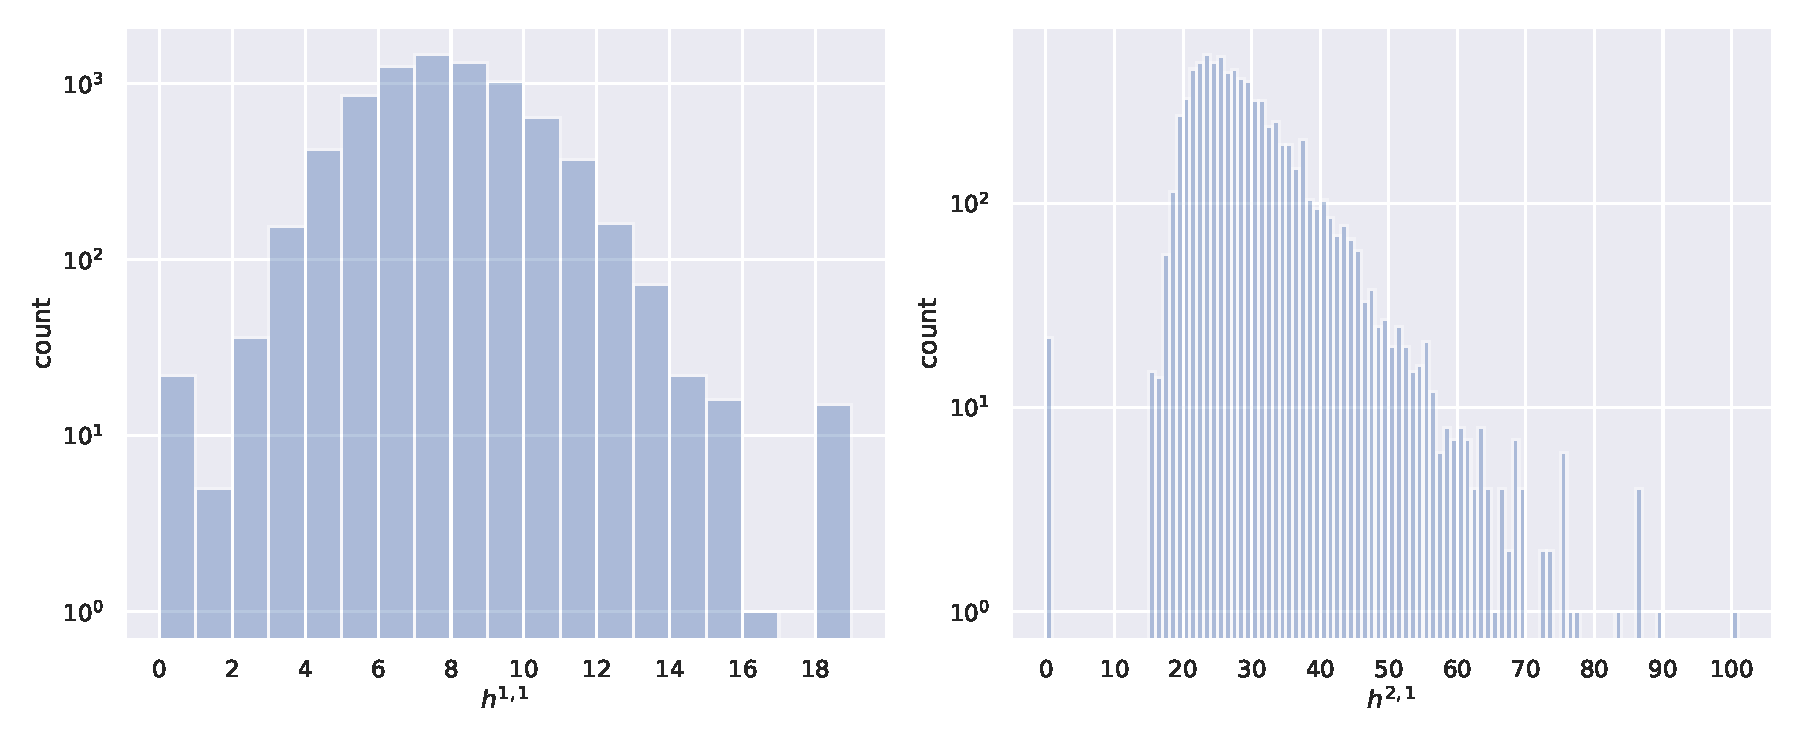
\includegraphics[width=\linewidth, trim={0 0.45in 6in 0}, clip]{img/label-distribution_orig}
    \caption{\hodge{1}{1}}
    \label{fig:data:hist-h11}
  \end{subfigure}
  \hfill
  \begin{subfigure}[c]{.45\linewidth}
    \centering
    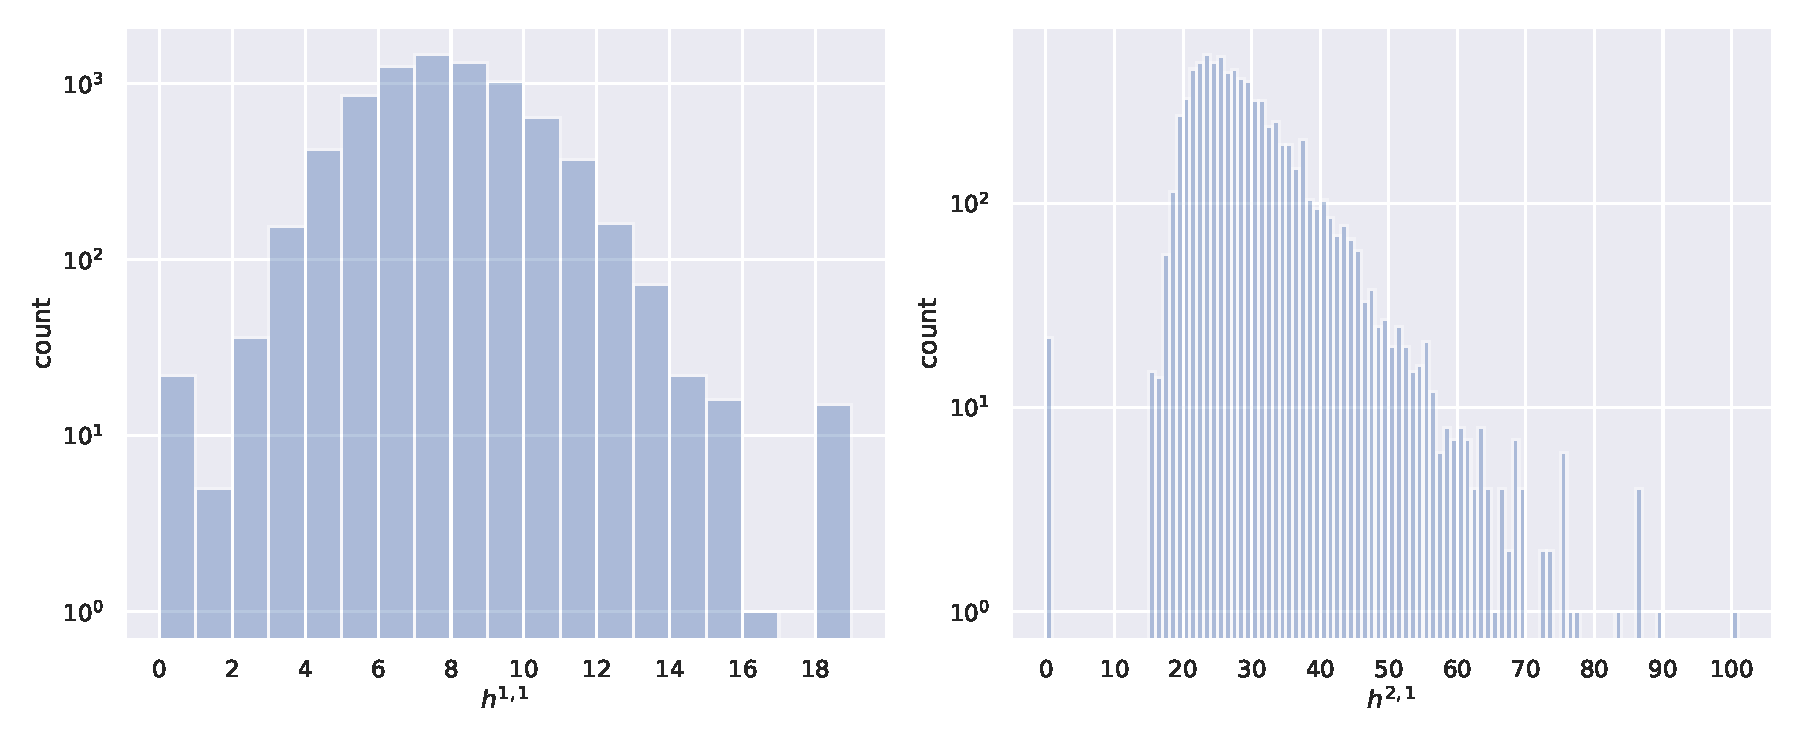
\includegraphics[width=\linewidth, trim={6in 0.45in 0 0}, clip]{img/label-distribution_orig}
    \caption{\hodge{2}{1}}
    \label{fig:data:hist-h21}
  \end{subfigure}
  \caption{Distribution of the Hodge numbers (log scale).}
  \label{fig:data:hist-hodge}
\end{figure}

The configuration matrix completely encodes the information of the \cicy and all topological quantities can be derived from it.
However the computations are involved and there is often no closed-form expression.
This situation is typical in algebraic geometry and it can be even worse for some problems, in the sense that it is not even known how to compute the desired quantity (e.g. the metric of \cy manifolds).
For these reasons it is interesting to study how to retrieve these properties using \ml algorithms.
In what follows we focus on the prediction of the Hodge numbers.
To provide a good test case for the use of \ml in context where the mathematical theory is not completely understood, we make no use of known formulas.


% vim: ft=tex
